\documentclass[11pt,a3paper,landscape]{article}
\usepackage[margin=1in]{geometry}
\usepackage{pgfgantt}
\usepackage{graphicx}
\usepackage{hyperref}
\usepackage{titlesec}
\usepackage{array}
\usepackage{booktabs}
\usepackage{fancyhdr}
\usepackage{lastpage}
\usepackage{xcolor}
\usepackage{longtable}
\usepackage{pdflscape}
\usepackage{afterpage}

% Color definitions
\definecolor{dreamlabblue}{RGB}{0,82,147}
\definecolor{dreamlabgreen}{RGB}{0,155,119}
\definecolor{dreamlabgray}{RGB}{128,128,128}
\definecolor{dreamlabyellow}{RGB}{255,193,7}
\definecolor{dreamlabred}{RGB}{220,53,69}

% Gantt chart styling
\ganttset{
    canvas/.style={draw=black!5, line width=.75pt},
    bar/.style={draw=dreamlabblue, fill=dreamlabblue!80},
    bar incomplete/.style={draw=dreamlabgreen, fill=dreamlabgreen!50},
    milestone/.style={draw=dreamlabred, fill=dreamlabred},
    group/.style={draw=black, fill=dreamlabgray!30},
    link/.style={->, thick, dreamlabblue}
}

% Header and footer
\pagestyle{fancy}
\fancyhf{}
\fancyhead[L]{\textcolor{dreamlabblue}{\textbf{DreamLab Implementation Timeline}}}
\fancyhead[R]{\textcolor{dreamlabblue}{Version 1.0}}
\fancyfoot[C]{Page \thepage\ of \pageref{LastPage}}
\renewcommand{\headrulewidth}{1pt}
\renewcommand{\footrulewidth}{0.5pt}

\begin{document}

\begin{titlepage}
\centering
\vspace*{2cm}
{\Huge\bfseries\color{dreamlabblue} DreamLab Project Timeline\par}
\vspace{1cm}
{\Large\color{dreamlabgreen} 18-Month Implementation Roadmap\par}
\vspace{3cm}
{\large\bfseries Gantt Charts and Resource Planning\par}
\vspace{0.5cm}
{\large January 2025 - June 2026\par}
\vfill
{\large\textit{From Vision to Reality: Structured Implementation Plan}\par}
\end{titlepage}

\section{Executive Summary}

This document presents the comprehensive 18-month implementation timeline for DreamLab's launch and scaling strategy. The timeline is structured across five major phases:

\begin{enumerate}
\item \textbf{Foundation Phase} (Months 1-3): Setup and preparation
\item \textbf{Pilot Phase} (Months 4-6): Initial program delivery
\item \textbf{Launch Phase} (Months 7-9): Full market entry
\item \textbf{Growth Phase} (Months 10-15): Scaling operations
\item \textbf{Optimization Phase} (Months 16-18): Refinement and expansion
\end{enumerate}

\section{Master Timeline Overview}

\subsection{Phase Gates and Decision Points}

\begin{longtable}{|p{3cm}|p{4cm}|p{6cm}|p{4cm}|}
\hline
\textbf{Phase Gate} & \textbf{Timeline} & \textbf{Success Criteria} & \textbf{Go/No-Go Decision} \\
\hline
\endhead
Foundation Complete & End of Month 3 & Facility ready, team hired, systems operational & Board Review \\
\hline
Pilot Success & End of Month 6 & 20+ participants, >90\% satisfaction & Investment Committee \\
\hline
Market Launch & End of Month 9 & 100+ enrolled, positive cash flow & Full Board Meeting \\
\hline
Growth Targets & End of Month 15 & 500+ participants, 3 locations & Strategic Review \\
\hline
Scale Decision & End of Month 18 & Profitability achieved, expansion ready & Investor Meeting \\
\hline
\end{longtable}

\newpage
\section{Detailed Gantt Charts}

\subsection{Foundation Phase (Months 1-3)}

\begin{ganttchart}[
    vgrid,
    hgrid,
    x unit=1.8cm,
    y unit title=0.6cm,
    y unit chart=0.5cm,
    time slot format=simple,
    title height=1,
    bar height=0.7,
    milestone height=0.5,
    title label font=\small,
    bar label font=\footnotesize,
    group label font=\small\bfseries
]{1}{12}
    \gantttitle{Foundation Phase - Q1 2025}{12} \\
    \gantttitlelist{1,...,12}{1} \\
    
    % Legal and Corporate Setup
    \ganttgroup{Legal \& Corporate}{1}{8} \\
    \ganttbar{Company Registration}{1}{2} \\
    \ganttbar{Legal Framework}{1}{4} \\
    \ganttbar{Insurance Setup}{3}{5} \\
    \ganttbar{Banking \& Finance}{2}{4} \\
    \ganttmilestone{Legal Complete}{8} \\
    
    % Facility Development
    \ganttgroup{Facility Setup}{2}{11} \\
    \ganttbar{Location Search}{2}{4} \\
    \ganttbar{Lease Negotiation}{4}{6} \\
    \ganttbar{Design \& Planning}{5}{7} \\
    \ganttbar{Renovation Works}{7}{10} \\
    \ganttbar{Equipment Install}{9}{11} \\
    \ganttmilestone{Facility Ready}{11} \\
    
    % Team Building
    \ganttgroup{Team Building}{1}{10} \\
    \ganttbar{Leadership Hire}{1}{4} \\
    \ganttbar{Core Team Recruit}{3}{7} \\
    \ganttbar{Instructor Search}{4}{8} \\
    \ganttbar{Training Program}{7}{10} \\
    \ganttmilestone{Team Operational}{10} \\
    
    % Technology Setup
    \ganttgroup{Technology}{3}{11} \\
    \ganttbar{Platform Selection}{3}{5} \\
    \ganttbar{System Development}{5}{9} \\
    \ganttbar{Integration}{8}{10} \\
    \ganttbar{Testing \& Launch}{9}{11} \\
    \ganttmilestone{Tech Go-Live}{11} \\
    
    % Marketing Preparation
    \ganttgroup{Marketing Prep}{2}{12} \\
    \ganttbar{Brand Development}{2}{5} \\
    \ganttbar{Website Design}{4}{7} \\
    \ganttbar{Content Creation}{6}{10} \\
    \ganttbar{Launch Campaign}{9}{12} \\
    
    % Links
    \ganttlink{elem3}{elem4}
    \ganttlink{elem7}{elem8}
    \ganttlink{elem12}{elem13}
\end{ganttchart}

\subsection{Pilot Phase (Months 4-6)}

\begin{ganttchart}[
    vgrid,
    hgrid,
    x unit=1.8cm,
    y unit title=0.6cm,
    y unit chart=0.5cm,
    time slot format=simple,
    title height=1,
    bar height=0.7,
    milestone height=0.5,
    title label font=\small,
    bar label font=\footnotesize,
    group label font=\small\bfseries
]{13}{24}
    \gantttitle{Pilot Phase - Q2 2025}{12} \\
    \gantttitlelist{13,...,24}{1} \\
    
    % Pilot Program Delivery
    \ganttgroup{Pilot Programs}{13}{24} \\
    \ganttbar{Cohort 1 Recruitment}{13}{15} \\
    \ganttbar{Cohort 1 Delivery}{16}{21} \\
    \ganttbar{Cohort 2 Recruitment}{17}{19} \\
    \ganttbar{Cohort 2 Delivery}{20}{24} \\
    \ganttmilestone{Pilot Complete}{24} \\
    
    % Quality Assurance
    \ganttgroup{Quality \& Feedback}{15}{24} \\
    \ganttbar{Feedback Systems}{15}{16} \\
    \ganttbar{Daily Monitoring}{16}{24} \\
    \ganttbar{Weekly Reviews}{16}{24} \\
    \ganttbar{Program Iteration}{18}{22} \\
    
    % Marketing Ramp-up
    \ganttgroup{Marketing Launch}{13}{24} \\
    \ganttbar{PR Campaign}{13}{16} \\
    \ganttbar{Digital Marketing}{14}{24} \\
    \ganttbar{Events \& Networking}{16}{24} \\
    \ganttbar{Partnership Dev}{15}{24} \\
    
    % Operations Refinement
    \ganttgroup{Operations}{13}{24} \\
    \ganttbar{Process Documentation}{13}{18} \\
    \ganttbar{Staff Development}{14}{24} \\
    \ganttbar{Vendor Optimization}{16}{20} \\
    \ganttbar{Cost Management}{15}{24} \\
    
    % Financial Management
    \ganttgroup{Finance}{13}{24} \\
    \ganttbar{Revenue Tracking}{16}{24} \\
    \ganttbar{Cost Analysis}{16}{24} \\
    \ganttbar{Investor Updates}{18}{18} \\
    \ganttbar{Funding Round Prep}{20}{24} \\
\end{ganttchart}

\subsection{Launch Phase (Months 7-9)}

\begin{ganttchart}[
    vgrid,
    hgrid,
    x unit=1.8cm,
    y unit title=0.6cm,
    y unit chart=0.5cm,
    time slot format=simple,
    title height=1,
    bar height=0.7,
    milestone height=0.5,
    title label font=\small,
    bar label font=\footnotesize,
    group label font=\small\bfseries
]{25}{36}
    \gantttitle{Launch Phase - Q3 2025}{12} \\
    \gantttitlelist{25,...,36}{1} \\
    
    % Full Program Launch
    \ganttgroup{Program Delivery}{25}{36} \\
    \ganttbar{Foundation Programs}{25}{36} \\
    \ganttbar{Accelerator Launch}{28}{36} \\
    \ganttbar{Executive Program}{31}{36} \\
    \ganttmilestone{All Programs Live}{36} \\
    
    % Scale Preparation
    \ganttgroup{Scaling Prep}{25}{36} \\
    \ganttbar{Second Location}{25}{32} \\
    \ganttbar{Team Expansion}{26}{30} \\
    \ganttbar{System Scaling}{28}{34} \\
    \ganttbar{Process Automation}{30}{36} \\
    
    % Market Expansion
    \ganttgroup{Market Growth}{25}{36} \\
    \ganttbar{B2B Sales Launch}{25}{36} \\
    \ganttbar{Corporate Partners}{27}{36} \\
    \ganttbar{Alumni Network}{28}{36} \\
    \ganttbar{Referral Program}{30}{36} \\
    
    % Quality Enhancement
    \ganttgroup{Quality}{25}{36} \\
    \ganttbar{Accreditation}{25}{34} \\
    \ganttbar{Curriculum v2.0}{28}{35} \\
    \ganttbar{Instructor Excellence}{26}{36} \\
    \ganttbar{Tech Enhancement}{30}{36} \\
    
    % Financial Growth
    \ganttgroup{Finance}{25}{36} \\
    \ganttbar{Series A Prep}{25}{30} \\
    \ganttbar{Revenue Growth}{25}{36} \\
    \ganttbar{Unit Economics}{28}{36} \\
    \ganttmilestone{Break-even}{36} \\
\end{ganttchart}

\subsection{Growth Phase (Months 10-15)}

\begin{ganttchart}[
    vgrid,
    hgrid,
    x unit=0.9cm,
    y unit title=0.6cm,
    y unit chart=0.5cm,
    time slot format=simple,
    title height=1,
    bar height=0.7,
    milestone height=0.5,
    title label font=\small,
    bar label font=\footnotesize,
    group label font=\small\bfseries
]{37}{60}
    \gantttitle{Growth Phase - Q4 2025 - Q2 2026}{24} \\
    \gantttitlelist{37,...,60}{1} \\
    
    % Geographic Expansion
    \ganttgroup{Expansion}{37}{60} \\
    \ganttbar{London Launch}{37}{48} \\
    \ganttbar{Edinburgh Prep}{43}{54} \\
    \ganttbar{Birmingham Prep}{49}{60} \\
    \ganttbar{International Planning}{52}{60} \\
    \ganttmilestone{3 Cities Operational}{54} \\
    
    % Program Development
    \ganttgroup{Programs}{37}{60} \\
    \ganttbar{Specialty Tracks}{37}{45} \\
    \ganttbar{Online Hybrid}{40}{50} \\
    \ganttbar{Corporate Custom}{43}{60} \\
    \ganttbar{Certification Launch}{46}{56} \\
    
    % Technology Scale
    \ganttgroup{Technology}{37}{60} \\
    \ganttbar{Platform v2.0}{37}{46} \\
    \ganttbar{Mobile Apps}{40}{48} \\
    \ganttbar{AI Integration}{45}{55} \\
    \ganttbar{Analytics Platform}{48}{58} \\
    
    % Team Growth
    \ganttgroup{Organization}{37}{60} \\
    \ganttbar{Leadership Team}{37}{42} \\
    \ganttbar{Regional Teams}{40}{52} \\
    \ganttbar{Center Excellence}{45}{60} \\
    \ganttbar{Culture Program}{37}{60} \\
    
    % Strategic Initiatives
    \ganttgroup{Strategy}{37}{60} \\
    \ganttbar{M\&A Opportunities}{45}{60} \\
    \ganttbar{Series B Funding}{48}{54} \\
    \ganttbar{IPO Preparation}{55}{60} \\
    \ganttmilestone{Funding Secured}{54} \\
\end{ganttchart}

\subsection{Optimization Phase (Months 16-18)}

\begin{ganttchart}[
    vgrid,
    hgrid,
    x unit=1.8cm,
    y unit title=0.6cm,
    y unit chart=0.5cm,
    time slot format=simple,
    title height=1,
    bar height=0.7,
    milestone height=0.5,
    title label font=\small,
    bar label font=\footnotesize,
    group label font=\small\bfseries
]{61}{72}
    \gantttitle{Optimization Phase - Q2-Q3 2026}{12} \\
    \gantttitlelist{61,...,72}{1} \\
    
    % Excellence Programs
    \ganttgroup{Excellence}{61}{72} \\
    \ganttbar{Quality Certification}{61}{66} \\
    \ganttbar{Awards \& Recognition}{63}{69} \\
    \ganttbar{Research Center}{64}{72} \\
    \ganttbar{Thought Leadership}{61}{72} \\
    
    % International Launch
    \ganttgroup{International}{61}{72} \\
    \ganttbar{Market Research}{61}{64} \\
    \ganttbar{Partner Selection}{63}{67} \\
    \ganttbar{Pilot Programs}{66}{72} \\
    \ganttbar{Global Platform}{65}{72} \\
    
    % Innovation
    \ganttgroup{Innovation}{61}{72} \\
    \ganttbar{R\&D Lab}{61}{72} \\
    \ganttbar{Tech Partnerships}{62}{70} \\
    \ganttbar{New Products}{65}{72} \\
    \ganttbar{Future Strategy}{68}{72} \\
    
    % Sustainability
    \ganttgroup{Sustainability}{61}{72} \\
    \ganttbar{ESG Framework}{61}{65} \\
    \ganttbar{Impact Measurement}{63}{72} \\
    \ganttbar{Community Programs}{65}{72} \\
    \ganttbar{Annual Report}{70}{72} \\
    
    \ganttmilestone{Phase Complete}{72} \\
\end{ganttchart}

\newpage
\section{Critical Path Analysis}

\subsection{Critical Path Elements}

The following activities form the critical path for DreamLab's successful launch:

\begin{longtable}{|p{1cm}|p{4cm}|p{2cm}|p{2cm}|p{6cm}|}
\hline
\textbf{ID} & \textbf{Activity} & \textbf{Duration} & \textbf{Start} & \textbf{Dependencies} \\
\hline
\endhead
CP1 & Legal Entity Setup & 2 weeks & Week 1 & None \\
\hline
CP2 & Facility Lease & 4 weeks & Week 3 & CP1 \\
\hline
CP3 & Core Team Hiring & 8 weeks & Week 1 & CP1 \\
\hline
CP4 & Facility Fit-out & 6 weeks & Week 7 & CP2 \\
\hline
CP5 & Technology Platform & 8 weeks & Week 5 & CP3 \\
\hline
CP6 & Instructor Recruitment & 8 weeks & Week 5 & CP3 \\
\hline
CP7 & Program Development & 6 weeks & Week 9 & CP6 \\
\hline
CP8 & Marketing Launch & 4 weeks & Week 11 & CP7 \\
\hline
CP9 & First Cohort & 2 weeks & Week 13 & CP4, CP5, CP7, CP8 \\
\hline
CP10 & Program Delivery & 8 weeks & Week 15 & CP9 \\
\hline
\end{longtable}

\subsection{Critical Path Visualization}

\begin{center}
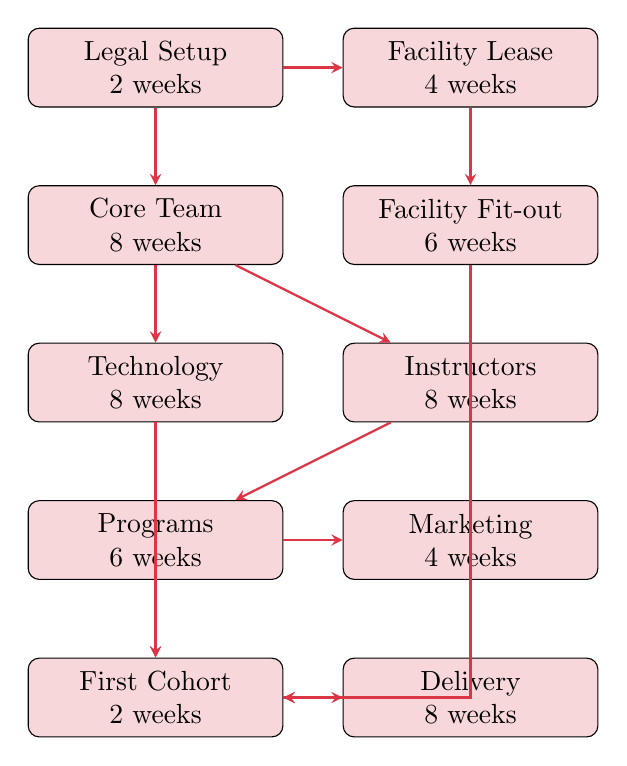
\begin{tikzpicture}[node distance=2cm, auto]
    % Define styles
    \tikzstyle{critical} = [rectangle, draw, fill=dreamlabred!20, text width=3cm, text centered, rounded corners, minimum height=1cm]
    \tikzstyle{arrow} = [thick,->,>=stealth,dreamlabred]
    
    % Nodes
    \node (cp1) [critical] {Legal Setup\\2 weeks};
    \node (cp2) [critical, right of=cp1, xshift=2cm] {Facility Lease\\4 weeks};
    \node (cp3) [critical, below of=cp1] {Core Team\\8 weeks};
    \node (cp4) [critical, right of=cp3, xshift=2cm] {Facility Fit-out\\6 weeks};
    \node (cp5) [critical, below of=cp3] {Technology\\8 weeks};
    \node (cp6) [critical, right of=cp5, xshift=2cm] {Instructors\\8 weeks};
    \node (cp7) [critical, below of=cp5] {Programs\\6 weeks};
    \node (cp8) [critical, right of=cp7, xshift=2cm] {Marketing\\4 weeks};
    \node (cp9) [critical, below of=cp7] {First Cohort\\2 weeks};
    \node (cp10) [critical, right of=cp9, xshift=2cm] {Delivery\\8 weeks};
    
    % Arrows
    \draw [arrow] (cp1) -- (cp2);
    \draw [arrow] (cp1) -- (cp3);
    \draw [arrow] (cp2) -- (cp4);
    \draw [arrow] (cp3) -- (cp5);
    \draw [arrow] (cp3) -- (cp6);
    \draw [arrow] (cp6) -- (cp7);
    \draw [arrow] (cp7) -- (cp8);
    \draw [arrow] (cp4) |- (cp9);
    \draw [arrow] (cp5) -- (cp9);
    \draw [arrow] (cp7) -- (cp9);
    \draw [arrow] (cp8) |- (cp9);
    \draw [arrow] (cp9) -- (cp10);
\end{tikzpicture}
\end{center}

\newpage
\section{Resource Allocation Matrix}

\subsection{Human Resources Allocation}

\begin{landscape}
\begin{longtable}{|p{3cm}|*{18}{c|}}
\hline
\textbf{Role/Resource} & \multicolumn{3}{c|}{\textbf{Q1 2025}} & \multicolumn{3}{c|}{\textbf{Q2 2025}} & \multicolumn{3}{c|}{\textbf{Q3 2025}} & \multicolumn{3}{c|}{\textbf{Q4 2025}} & \multicolumn{3}{c|}{\textbf{Q1 2026}} & \multicolumn{3}{c|}{\textbf{Q2 2026}} \\
\cline{2-19}
& M1 & M2 & M3 & M4 & M5 & M6 & M7 & M8 & M9 & M10 & M11 & M12 & M13 & M14 & M15 & M16 & M17 & M18 \\
\hline
\endhead
CEO & 1 & 1 & 1 & 1 & 1 & 1 & 1 & 1 & 1 & 1 & 1 & 1 & 1 & 1 & 1 & 1 & 1 & 1 \\
\hline
COO & 0 & 1 & 1 & 1 & 1 & 1 & 1 & 1 & 1 & 1 & 1 & 1 & 1 & 1 & 1 & 1 & 1 & 1 \\
\hline
CFO & 0 & 0 & 1 & 1 & 1 & 1 & 1 & 1 & 1 & 1 & 1 & 1 & 1 & 1 & 1 & 1 & 1 & 1 \\
\hline
Program Directors & 0 & 0 & 1 & 2 & 2 & 2 & 3 & 3 & 3 & 4 & 4 & 4 & 5 & 5 & 5 & 6 & 6 & 6 \\
\hline
Lead Instructors & 0 & 0 & 0 & 2 & 4 & 4 & 6 & 8 & 8 & 10 & 12 & 12 & 15 & 15 & 15 & 18 & 18 & 20 \\
\hline
Support Instructors & 0 & 0 & 0 & 2 & 4 & 6 & 8 & 10 & 12 & 15 & 18 & 20 & 25 & 28 & 30 & 35 & 38 & 40 \\
\hline
Sales Team & 0 & 1 & 2 & 3 & 4 & 4 & 5 & 6 & 6 & 8 & 10 & 10 & 12 & 14 & 15 & 18 & 20 & 20 \\
\hline
Marketing Team & 1 & 2 & 2 & 3 & 3 & 4 & 4 & 5 & 5 & 6 & 7 & 8 & 10 & 10 & 12 & 15 & 15 & 15 \\
\hline
Operations Team & 1 & 2 & 3 & 4 & 5 & 5 & 6 & 7 & 8 & 10 & 12 & 12 & 15 & 18 & 20 & 25 & 28 & 30 \\
\hline
Technology Team & 0 & 1 & 2 & 3 & 4 & 4 & 5 & 5 & 6 & 8 & 8 & 10 & 12 & 12 & 15 & 18 & 20 & 20 \\
\hline
Finance Team & 1 & 1 & 2 & 2 & 3 & 3 & 4 & 4 & 4 & 5 & 5 & 6 & 8 & 8 & 10 & 12 & 12 & 12 \\
\hline
HR Team & 0 & 1 & 1 & 2 & 2 & 2 & 3 & 3 & 3 & 4 & 4 & 5 & 6 & 6 & 8 & 10 & 10 & 10 \\
\hline
\textbf{Total FTE} & 4 & 10 & 16 & 26 & 35 & 38 & 48 & 55 & 59 & 75 & 86 & 92 & 114 & 120 & 134 & 159 & 168 & 175 \\
\hline
\end{longtable}
\end{landscape}

\subsection{Financial Resource Allocation}

\begin{longtable}{|p{4cm}|*{6}{r|}}
\hline
\textbf{Budget Category} & \textbf{Q1 2025} & \textbf{Q2 2025} & \textbf{Q3 2025} & \textbf{Q4 2025} & \textbf{Q1 2026} & \textbf{Q2 2026} \\
\hline
\endhead
\multicolumn{7}{|l|}{\textbf{Capital Expenditure}} \\
\hline
Facility Setup & £500,000 & £200,000 & £300,000 & £400,000 & £500,000 & £300,000 \\
\hline
Technology Platform & £200,000 & £150,000 & £100,000 & £150,000 & £200,000 & £250,000 \\
\hline
Equipment \& Furniture & £150,000 & £50,000 & £100,000 & £150,000 & £200,000 & £100,000 \\
\hline
\textbf{Subtotal CapEx} & £850,000 & £400,000 & £500,000 & £700,000 & £900,000 & £650,000 \\
\hline
\multicolumn{7}{|l|}{\textbf{Operating Expenditure}} \\
\hline
Staff Costs & £120,000 & £350,000 & £450,000 & £690,000 & £1,020,000 & £1,260,000 \\
\hline
Marketing \& Sales & £100,000 & £200,000 & £300,000 & £400,000 & £500,000 & £600,000 \\
\hline
Facility Operations & £50,000 & £75,000 & £100,000 & £150,000 & £200,000 & £250,000 \\
\hline
Program Delivery & £0 & £100,000 & £200,000 & £300,000 & £450,000 & £600,000 \\
\hline
Technology \& Systems & £30,000 & £50,000 & £75,000 & £100,000 & £150,000 & £200,000 \\
\hline
Professional Services & £50,000 & £40,000 & £50,000 & £60,000 & £80,000 & £100,000 \\
\hline
\textbf{Subtotal OpEx} & £350,000 & £815,000 & £1,175,000 & £1,700,000 & £2,400,000 & £3,010,000 \\
\hline
\textbf{Total Quarterly Spend} & £1,200,000 & £1,215,000 & £1,675,000 & £2,400,000 & £3,300,000 & £3,660,000 \\
\hline
\textbf{Cumulative Spend} & £1,200,000 & £2,415,000 & £4,090,000 & £6,490,000 & £9,790,000 & £13,450,000 \\
\hline
\end{longtable}

\newpage
\section{Dependency Mapping}

\subsection{Major Dependencies Matrix}

\begin{center}
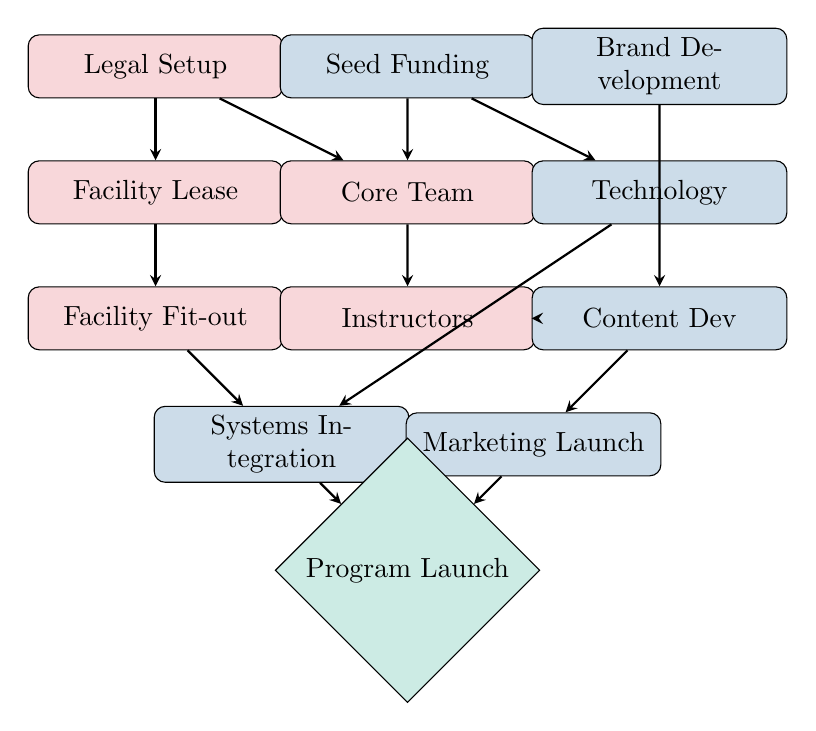
\begin{tikzpicture}[scale=0.8]
    % Define styles
    \tikzstyle{task} = [rectangle, draw, fill=dreamlabblue!20, text width=3cm, text centered, rounded corners, minimum height=0.8cm]
    \tikzstyle{critical} = [rectangle, draw, fill=dreamlabred!20, text width=3cm, text centered, rounded corners, minimum height=0.8cm]
    \tikzstyle{milestone} = [diamond, draw, fill=dreamlabgreen!20, text centered, minimum height=1cm, minimum width=1cm]
    \tikzstyle{arrow} = [thick,->,>=stealth]
    
    % Layer 1
    \node (legal) [critical] at (0,0) {Legal Setup};
    \node (funding) [task] at (4,0) {Seed Funding};
    \node (brand) [task] at (8,0) {Brand Development};
    
    % Layer 2
    \node (facility) [critical] at (0,-2) {Facility Lease};
    \node (team) [critical] at (4,-2) {Core Team};
    \node (tech) [task] at (8,-2) {Technology};
    
    % Layer 3
    \node (fitout) [critical] at (0,-4) {Facility Fit-out};
    \node (instructors) [critical] at (4,-4) {Instructors};
    \node (content) [task] at (8,-4) {Content Dev};
    
    % Layer 4
    \node (systems) [task] at (2,-6) {Systems Integration};
    \node (marketing) [task] at (6,-6) {Marketing Launch};
    
    % Milestone
    \node (launch) [milestone] at (4,-8) {Program Launch};
    
    % Dependencies
    \draw [arrow] (legal) -- (facility);
    \draw [arrow] (legal) -- (team);
    \draw [arrow] (funding) -- (team);
    \draw [arrow] (funding) -- (tech);
    \draw [arrow] (facility) -- (fitout);
    \draw [arrow] (team) -- (instructors);
    \draw [arrow] (brand) -- (content);
    \draw [arrow] (tech) -- (systems);
    \draw [arrow] (instructors) -- (content);
    \draw [arrow] (content) -- (marketing);
    \draw [arrow] (fitout) -- (systems);
    \draw [arrow] (systems) -- (launch);
    \draw [arrow] (marketing) -- (launch);
\end{tikzpicture}
\end{center}

\subsection{Risk Dependencies}

\begin{longtable}{|p{3cm}|p{4cm}|p{3cm}|p{4cm}|}
\hline
\textbf{Activity} & \textbf{Dependencies} & \textbf{Risk Level} & \textbf{Mitigation Strategy} \\
\hline
\endhead
Facility Fit-out & Lease Agreement, Permits & High & Early permit applications, contingency venue \\
\hline
First Cohort & All critical path items & Critical & Soft launch option, phased enrollment \\
\hline
Technology Platform & Vendor selection, Integration & Medium & Multiple vendor options, agile development \\
\hline
Instructor Recruitment & Market availability, Budget & High & Pipeline building, competitive packages \\
\hline
Accreditation & Program design, Evidence & Medium & Early engagement, consultant support \\
\hline
Series A Funding & Financial performance, Growth & High & Multiple investor engagement, bridge options \\
\hline
\end{longtable}

\newpage
\section{Risk Mitigation Timeline}

\subsection{Risk Register and Mitigation Schedule}

\begin{ganttchart}[
    vgrid,
    hgrid,
    x unit=0.8cm,
    y unit title=0.6cm,
    y unit chart=0.5cm,
    time slot format=simple,
    title height=1,
    bar height=0.6,
    title label font=\small,
    bar label font=\footnotesize,
    group label font=\small\bfseries,
    bar/.append style={fill=dreamlabred!60},
    group/.append style={fill=dreamlabyellow!30}
]{1}{18}
    \gantttitle{Risk Mitigation Timeline - 18 Months}{18} \\
    \gantttitlelist{1,...,18}{1} \\
    
    % Strategic Risks
    \ganttgroup{Strategic Risks}{1}{18} \\
    \ganttbar{Market Competition}{1}{18} \\
    \ganttbar{Economic Downturn}{1}{18} \\
    \ganttbar{Regulatory Changes}{3}{15} \\
    
    % Operational Risks
    \ganttgroup{Operational Risks}{1}{18} \\
    \ganttbar{Facility Delays}{1}{6} \\
    \ganttbar{Technology Failure}{3}{12} \\
    \ganttbar{Quality Issues}{4}{18} \\
    \ganttbar{Scalability}{7}{18} \\
    
    % Financial Risks
    \ganttgroup{Financial Risks}{1}{18} \\
    \ganttbar{Funding Shortfall}{1}{9} \\
    \ganttbar{Cash Flow}{4}{18} \\
    \ganttbar{Cost Overrun}{1}{12} \\
    
    % People Risks
    \ganttgroup{People Risks}{1}{18} \\
    \ganttbar{Key Person Loss}{1}{18} \\
    \ganttbar{Talent Shortage}{3}{15} \\
    \ganttbar{Culture Dilution}{7}{18} \\
    
    % Market Risks
    \ganttgroup{Market Risks}{1}{18} \\
    \ganttbar{Demand Variability}{4}{18} \\
    \ganttbar{Brand Damage}{4}{18} \\
    \ganttbar{Partner Failure}{6}{18} \\
\end{ganttchart}

\subsection{Mitigation Action Timeline}

\begin{longtable}{|p{2cm}|p{3cm}|p{8cm}|p{2cm}|}
\hline
\textbf{Month} & \textbf{Risk Category} & \textbf{Mitigation Actions} & \textbf{Owner} \\
\hline
\endhead
1-3 & Financial & Secure seed funding, establish credit facilities, weekly cash monitoring & CFO \\
\hline
1-3 & Operational & Identify backup venues, create redundancy in critical systems & COO \\
\hline
4-6 & People & Implement retention bonuses, establish succession planning & HR Director \\
\hline
4-6 & Quality & Develop comprehensive QA framework, pilot testing protocols & Quality Lead \\
\hline
7-9 & Market & Launch brand protection strategy, diversify marketing channels & CMO \\
\hline
7-9 & Strategic & Competitive analysis, scenario planning workshops & CEO \\
\hline
10-12 & Scalability & Automate core processes, establish regional management structure & COO \\
\hline
13-15 & Financial & Series A preparation, alternative funding sources identified & CFO \\
\hline
16-18 & All Categories & Comprehensive risk review, update mitigation strategies & Risk Committee \\
\hline
\end{longtable}

\newpage
\section{Implementation Milestones}

\subsection{Key Milestones and Success Metrics}

\begin{longtable}{|p{1cm}|p{3cm}|p{3cm}|p{6cm}|p{2cm}|}
\hline
\textbf{ID} & \textbf{Milestone} & \textbf{Target Date} & \textbf{Success Criteria} & \textbf{Status} \\
\hline
\endhead
M1 & Company Incorporation & Week 2 & Legal entity established, bank accounts open & Pending \\
\hline
M2 & Seed Funding Closed & Week 4 & £2M raised, investor agreements signed & Pending \\
\hline
M3 & Manchester Facility & Week 12 & Lease signed, fit-out complete & Pending \\
\hline
M4 & Core Team Complete & Week 12 & 10 key positions filled & Pending \\
\hline
M5 & Technology Launch & Week 14 & Platform operational, tested with 100 users & Pending \\
\hline
M6 & First Cohort Start & Week 16 & 20+ participants enrolled, 95\% attendance & Pending \\
\hline
M7 & Pilot Completion & Week 26 & 90\% completion rate, NPS >70 & Pending \\
\hline
M8 & Full Launch & Week 28 & 3 programs running, 100+ participants & Pending \\
\hline
M9 & Break-even & Week 39 & Monthly revenue exceeds costs & Pending \\
\hline
M10 & Second Location & Week 45 & London facility operational & Pending \\
\hline
M11 & Series A Funding & Week 52 & £10M raised at £50M valuation & Pending \\
\hline
M12 & 500 Participants & Week 60 & Active enrollment target achieved & Pending \\
\hline
M13 & International Launch & Week 65 & First international cohort started & Pending \\
\hline
M14 & Profitability & Week 72 & Sustainable profit margins achieved & Pending \\
\hline
\end{longtable}

\subsection{Milestone Interdependencies}

\begin{center}
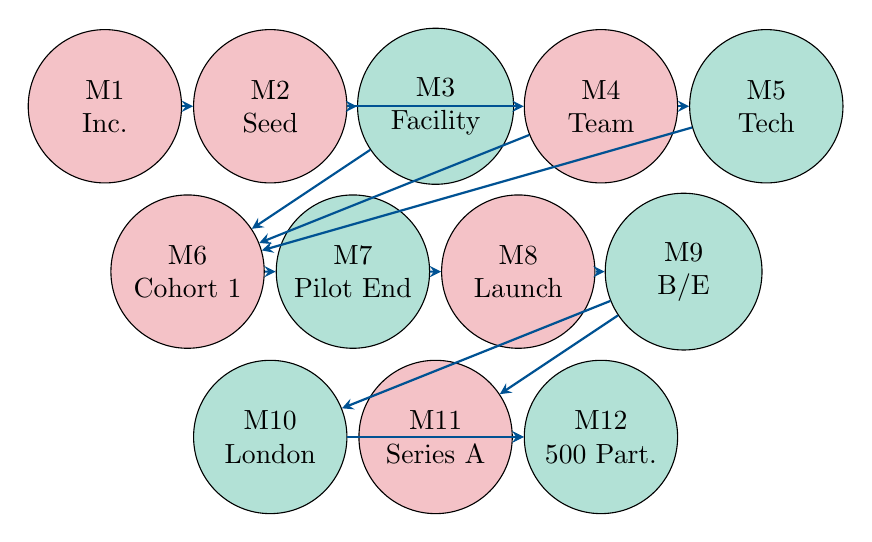
\begin{tikzpicture}[scale=0.7]
    % Define styles  
    \tikzstyle{milestone} = [circle, draw, fill=dreamlabgreen!30, text width=1.5cm, text centered, minimum height=1.5cm]
    \tikzstyle{critical} = [circle, draw, fill=dreamlabred!30, text width=1.5cm, text centered, minimum height=1.5cm]
    \tikzstyle{arrow} = [thick,->,>=stealth,dreamlabblue]
    
    % Create nodes in a timeline layout
    \node (m1) [critical] at (0,0) {M1\\Inc.};
    \node (m2) [critical] at (3,0) {M2\\Seed};
    \node (m3) [milestone] at (6,0) {M3\\Facility};
    \node (m4) [critical] at (9,0) {M4\\Team};
    \node (m5) [milestone] at (12,0) {M5\\Tech};
    
    \node (m6) [critical] at (1.5,-3) {M6\\Cohort 1};
    \node (m7) [milestone] at (4.5,-3) {M7\\Pilot End};
    \node (m8) [critical] at (7.5,-3) {M8\\Launch};
    \node (m9) [milestone] at (10.5,-3) {M9\\B/E};
    
    \node (m10) [milestone] at (3,-6) {M10\\London};
    \node (m11) [critical] at (6,-6) {M11\\Series A};
    \node (m12) [milestone] at (9,-6) {M12\\500 Part.};
    
    % Draw dependencies
    \draw [arrow] (m1) -- (m2);
    \draw [arrow] (m2) -- (m3);
    \draw [arrow] (m2) -- (m4);
    \draw [arrow] (m3) -- (m6);
    \draw [arrow] (m4) -- (m5);
    \draw [arrow] (m4) -- (m6);
    \draw [arrow] (m5) -- (m6);
    \draw [arrow] (m6) -- (m7);
    \draw [arrow] (m7) -- (m8);
    \draw [arrow] (m8) -- (m9);
    \draw [arrow] (m9) -- (m10);
    \draw [arrow] (m9) -- (m11);
    \draw [arrow] (m10) -- (m12);
    \draw [arrow] (m11) -- (m12);
\end{tikzpicture}
\end{center}

\newpage
\section{Resource Loading Charts}

\subsection{Monthly Resource Requirements}

\begin{center}
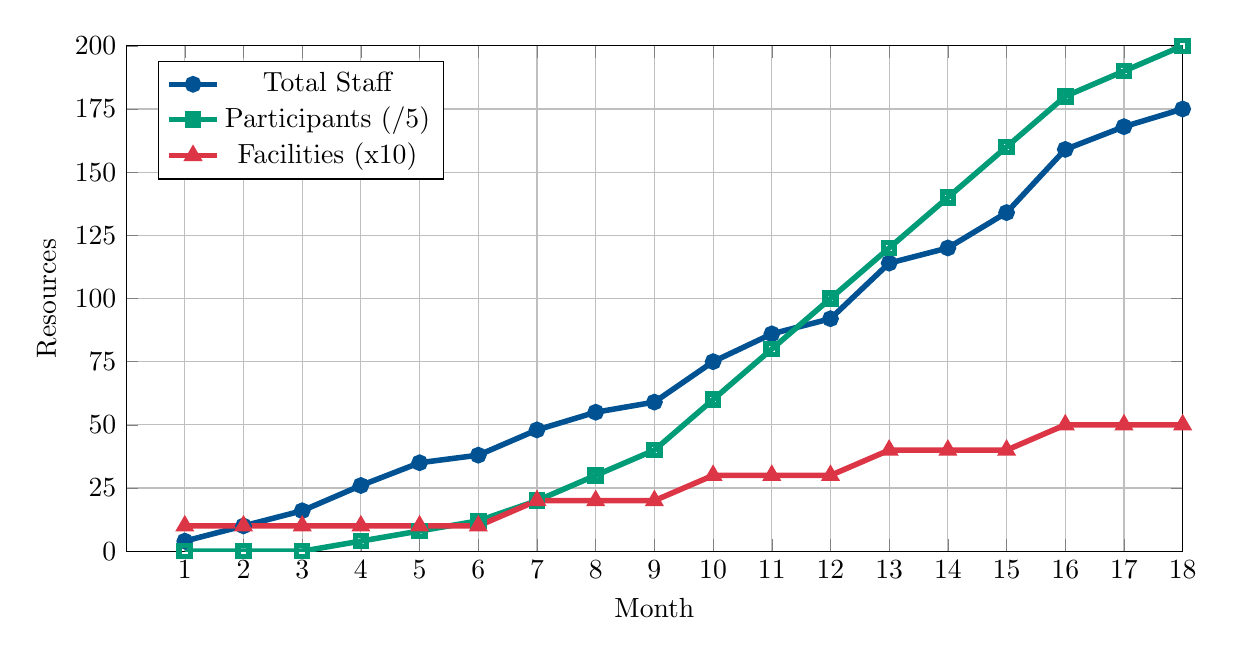
\begin{tikzpicture}
    \begin{axis}[
        width=15cm,
        height=8cm,
        xlabel={Month},
        ylabel={Resources},
        legend pos=north west,
        grid=major,
        xmin=0, xmax=18,
        ymin=0, ymax=200,
        xtick={1,2,3,4,5,6,7,8,9,10,11,12,13,14,15,16,17,18},
        ytick={0,25,50,75,100,125,150,175,200},
    ]
    
    % Staff headcount
    \addplot[color=dreamlabblue, line width=2pt, mark=*] coordinates {
        (1,4) (2,10) (3,16) (4,26) (5,35) (6,38) (7,48) (8,55) (9,59)
        (10,75) (11,86) (12,92) (13,114) (14,120) (15,134) (16,159) (17,168) (18,175)
    };
    \addlegendentry{Total Staff}
    
    % Participant numbers (scaled down by 5 for visualization)
    \addplot[color=dreamlabgreen, line width=2pt, mark=square] coordinates {
        (1,0) (2,0) (3,0) (4,4) (5,8) (6,12) (7,20) (8,30) (9,40)
        (10,60) (11,80) (12,100) (13,120) (14,140) (15,160) (16,180) (17,190) (18,200)
    };
    \addlegendentry{Participants (/5)}
    
    % Facilities (scaled by 10)
    \addplot[color=dreamlabred, line width=2pt, mark=triangle] coordinates {
        (1,10) (2,10) (3,10) (4,10) (5,10) (6,10) (7,20) (8,20) (9,20)
        (10,30) (11,30) (12,30) (13,40) (14,40) (15,40) (16,50) (17,50) (18,50)
    };
    \addlegendentry{Facilities (x10)}
    
    \end{axis}
\end{tikzpicture}
\end{center}

\subsection{Budget Burn Rate}

\begin{center}
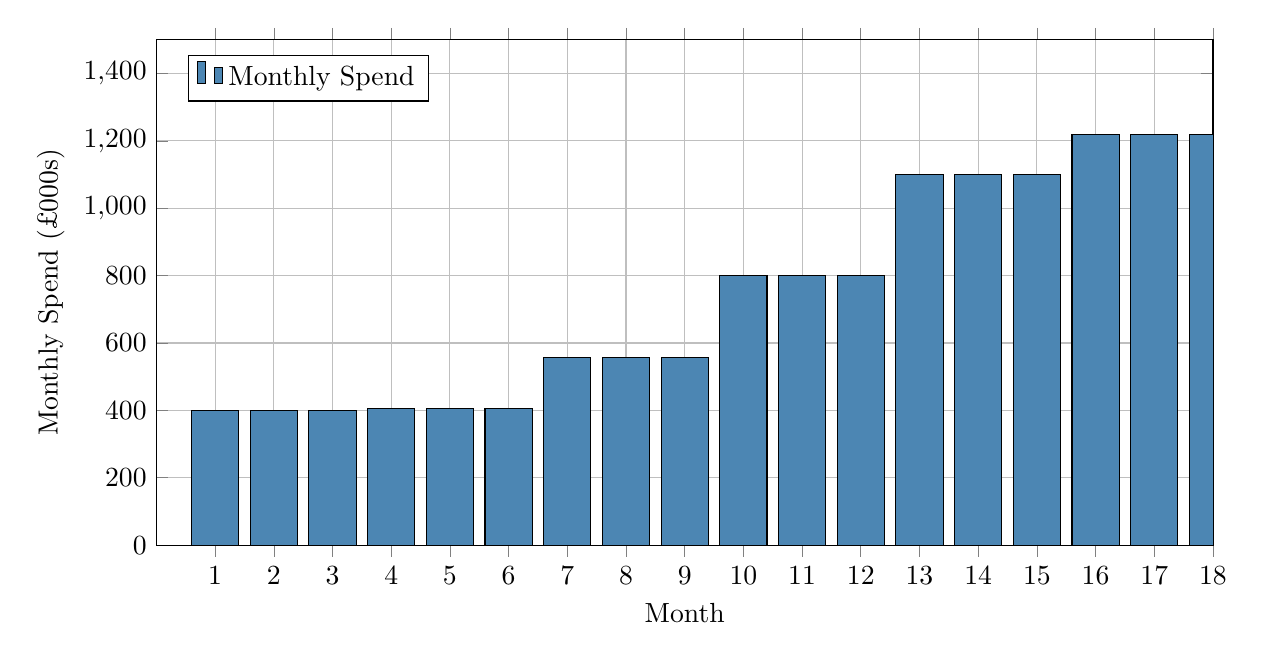
\begin{tikzpicture}
    \begin{axis}[
        width=15cm,
        height=8cm,
        xlabel={Month},
        ylabel={Monthly Spend (£000s)},
        legend pos=north west,
        grid=major,
        xmin=0, xmax=18,
        ymin=0, ymax=1500,
        xtick={1,2,3,4,5,6,7,8,9,10,11,12,13,14,15,16,17,18},
        ybar,
        bar width=0.6cm,
    ]
    
    % Monthly spend
    \addplot[fill=dreamlabblue!70] coordinates {
        (1,400) (2,400) (3,400) (4,405) (5,405) (6,405)
        (7,558) (8,558) (9,558) (10,800) (11,800) (12,800)
        (13,1100) (14,1100) (15,1100) (16,1220) (17,1220) (18,1220)
    };
    \addlegendentry{Monthly Spend}
    
    \end{axis}
\end{tikzpicture}
\end{center}

\newpage
\section{Conclusion and Next Steps}

\subsection{Implementation Success Factors}

\begin{enumerate}
\item \textbf{Critical Path Management}
   \begin{itemize}
   \item Weekly monitoring of critical activities
   \item Proactive issue resolution
   \item Resource reallocation as needed
   \end{itemize}

\item \textbf{Stakeholder Communication}
   \begin{itemize}
   \item Monthly investor updates
   \item Weekly team meetings
   \item Daily operational briefings
   \end{itemize}

\item \textbf{Risk Mitigation}
   \begin{itemize}
   \item Monthly risk reviews
   \item Contingency plan activation triggers
   \item Regular scenario planning
   \end{itemize}

\item \textbf{Quality Assurance}
   \begin{itemize}
   \item Phase gate reviews
   \item Continuous improvement cycles
   \item Customer feedback integration
   \end{itemize}
\end{enumerate}

\subsection{Immediate Next Steps}

\begin{longtable}{|p{1cm}|p{4cm}|p{3cm}|p{3cm}|p{3cm}|}
\hline
\textbf{Week} & \textbf{Action Item} & \textbf{Owner} & \textbf{Deliverable} & \textbf{Success Metric} \\
\hline
\endhead
1 & Finalize incorporation documents & CEO & Legal entity & Company registered \\
\hline
1 & Launch recruitment website & HR Director & Careers page & 50+ applications \\
\hline
2 & Investor meetings & CFO & Term sheets & 3+ offers \\
\hline
2 & Facility viewings & COO & Shortlist & 5 options \\
\hline
3 & Technology RFP & CTO & Vendor proposals & 3+ responses \\
\hline
3 & Brand agency selection & CMO & Agency contract & Brand workshop scheduled \\
\hline
4 & Core team interviews & CEO/COO & Offer letters & 5+ acceptances \\
\hline
4 & Funding close & CFO & Bank transfer & £2M received \\
\hline
\end{longtable}

\subsection{Project Governance}

\textbf{Steering Committee:}
\begin{itemize}
\item Weekly meetings during foundation phase
\item Bi-weekly during pilot phase
\item Monthly during growth phase
\item Quarterly during optimization phase
\end{itemize}

\textbf{Reporting Structure:}
\begin{itemize}
\item Daily operational updates
\item Weekly progress reports
\item Monthly board updates
\item Quarterly investor reviews
\end{itemize}

\textbf{Decision Authority:}
\begin{itemize}
\item CEO: Strategic decisions, >£100k commitments
\item COO: Operational decisions, <£100k commitments
\item Department Heads: Tactical decisions, <£25k
\item Team Leads: Day-to-day decisions, <£5k
\end{itemize}

\end{document}